\chapter{Discussion} \label{chapter:discussion}

% \newgeometry{margin=1.5in,left=1.5in,right=1.5in}

% 결과를 해석하고 기존 연구 결과들과의 일치성, 차별성 등을 제시하면서 본 논문의 결과가 전체적으로 이미 알려진 연구에 어떠한 정보내지는 새로운 해석을 제시하는 지 자유롭게 기술한다.

% 리뷰 논문의 경우 본 리뷰를 통해 얻은 주제의 현재와 앞으로의 전망 또는 연구 방향을 자유롭게 제시한다.

In this chapter we applied \texttt{Petasearch} to conduct two explorative analyses to show the effectiveness of the algorithm. Since \texttt{Petasearch} is capable of dealing with enormous datasets, we collected a large number of protein sequences including the ones assembled and compiled by the Serratus team \cite{edgar_petabase-scale_2022}
and the colabfold team \cite{mirdita_colabfold_2022}.
In the meantime, we also self-assembled terabyte-scale metagenomic data using PLASS \cite{steinegger_protein-level_2019}. In combination with the forementioned SRC and MERC data, we collected a total of nearly 10TB protein sequences. We then ran \texttt{Petasearch} on the collected data to search for \textbf{(1)} new short candidates of Cas 7-11 enzymes and \textbf{(2)} homologs for rare RNA virus protein with no known homologs in existing databases. The results of the two analyses were shown in \cref{section:find-new-candidates-of-cas-7-11-enzymes} and \cref{section:discover-homologs-for-rare-rna-virus-protein}.

\section{Find new candidates of Cas 7-11 enzymes} \label{section:find-new-candidates-of-cas-7-11-enzymes}

The CRISPR-Cas system is a powerful gene editing tool medidated by the Cas effector nucleases. Cas7-11 is a very short single-protein effector in class 1 CRISPR-Cas systems, thus showing almost no collateral activity and cell toxicity \cite{ozcan_programmable_2021}
We used \texttt{Petasearch} to search the Cas 7-11 MSA in \cite{ozcan_programmable_2021}
for new shorter candidates of Cas 7-11 enzymes in the collected data.

As a result, a total of 4484 valid Cas enzymes with at least one annotated putative catalytic domain were found. Amongst these, more than 300 even shorter (< 2000 amino acids long) sequences were found. The total searching time was no more than 10 minutes. The Multiple Sequence Alignment (MSA) of the short candidates were generated using \texttt{mafft} \cite{katoh_mafft_2013} and visualized usng \texttt{CIAlign} \cite{tumescheit_cialign_2022} in \cref{fig:cas7-11-candidate-MSA}. Those candidates could serve as a basis for future programmable editing tools.

\section{Discover homologs for rare RNA viral protein} \label{section:discover-homologs-for-rare-rna-virus-protein}

We searched the collected data with 6 RNA-dependent RNA polymerases (RdRPs) from different RNA viruses. There were no known homologs found in previously established databases for those RdRPs. Using \texttt{Petasearch}, we found at least 40 homologs each except for one RdRP which is only 100 amino acid long. The total amount of search time was no more than 8 minutes. The MSAs for each virus were visualized in \autoref{fig:rna-virus-hits}. Finding homologs for those rare RdRPs will enable structure predictors like AlphaFold2 to provide more accurate structure predictions, improving our understanding of those proteins.

\section{Conclusion and future work} \label{section:conclusion-and-future-work}

In \cref{chapter:results}, we showed that the optimizations for \texttt{Petasearch} prototype were proved to be successful. The algorithm currently strikes a good balance between space usage and speed, in the meantime provides competitive sensitivity in its designed applications at a much accelerated speed. In the two explorative analyses, the algorithm showed its capability in fast discovery of various new protein homologs in environmental metagenomic databases. We can conclude that \texttt{Petasearch} is a lightning fast searching algorithm that can enable researchers to explore the vast amount of evolutionary information available in current and upcoming databases.

For future directions, it will be beneficial to build a web service to make \texttt{Petasearch} more accessible to the public. We also plan to continuously integrate new metagenomic sequences to the current sequence corpus, making \texttt{Petasearch} able to explore a larger protein universe. We hope that \texttt{Petasearch} will become a valuable resource to uncover proteins for scientific,
medical and biotechnological purposes by making all-encompassing searches through environmental sequencing data possible for the first time.


\pagebreak
\clearpage
\begin{figpage}
  \newgeometry{left=8mm,right=8mm, bottom=15mm}
  \captionsetup[figure]{width=0.8\textwidth}
  \begin{figure}
    \centering
    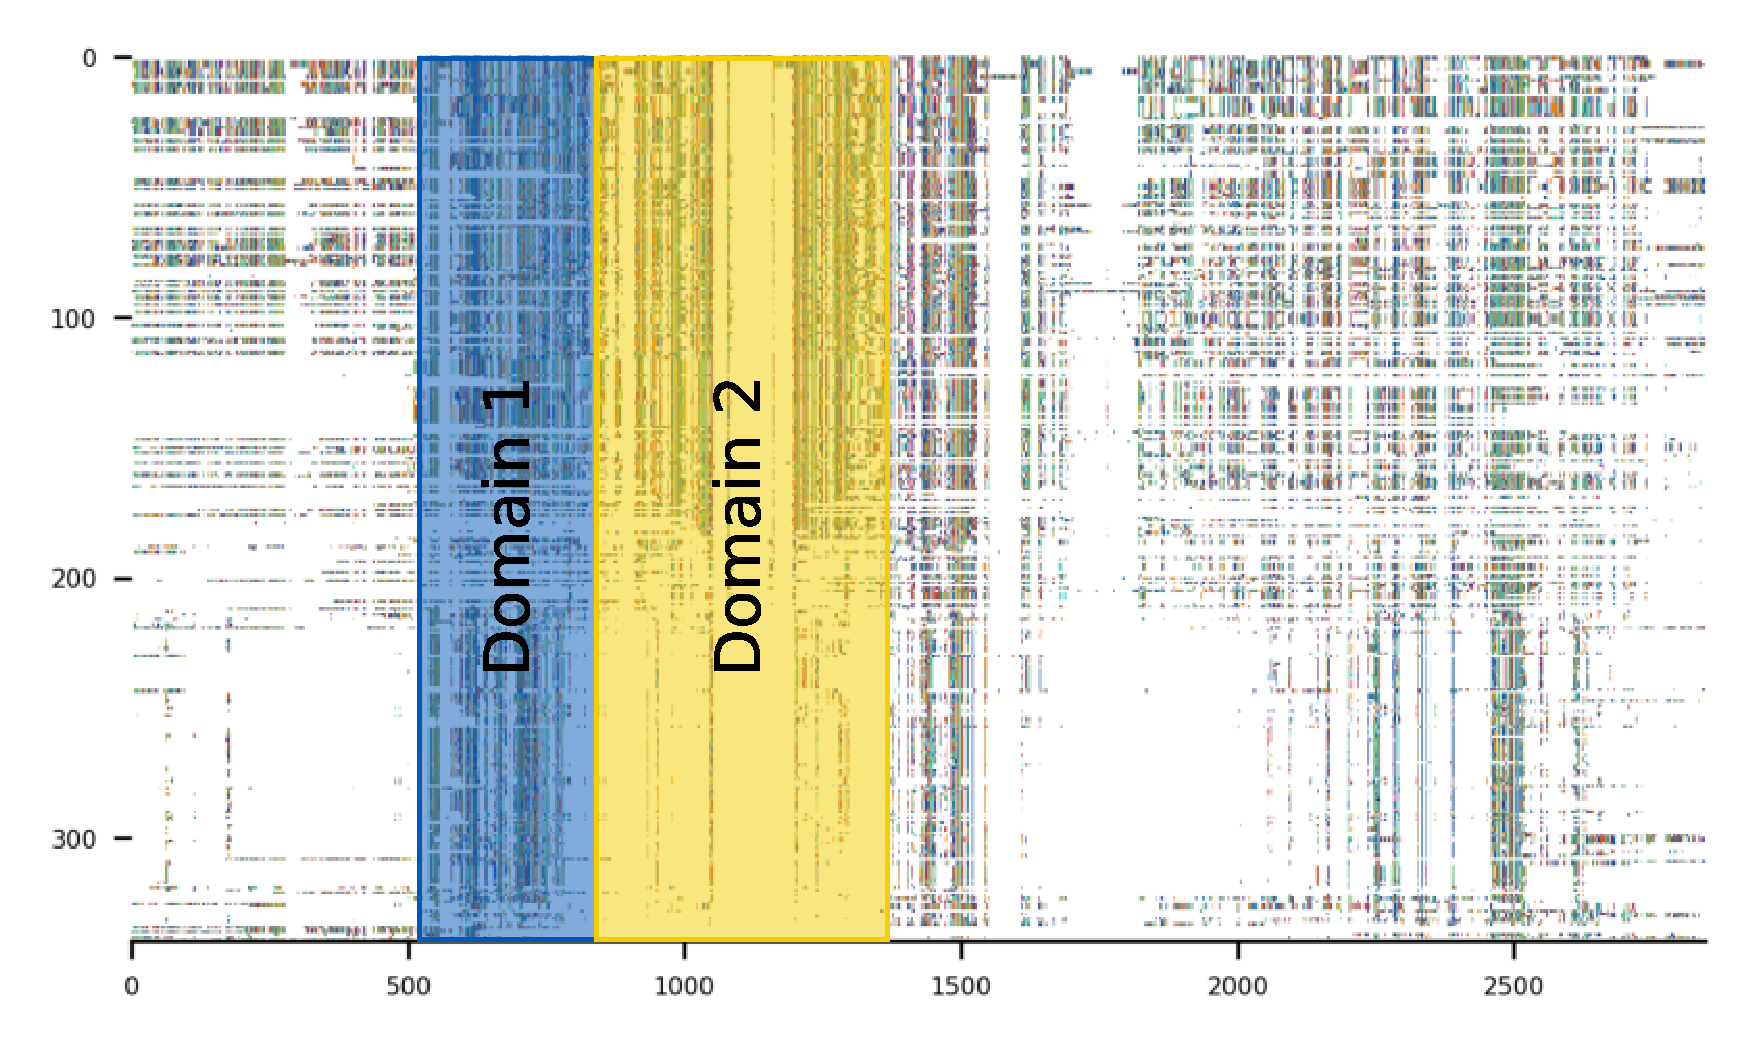
\includegraphics[width=0.8\textwidth]{images/cas711verysmall_valid_output.pdf}
    \caption{\textbf{Multiple Sequence Alignments of short (< 2000 amino acid) Cas7-11 candidates.} Domain 1 and domain 2 are putative catalytic domains of Cas7-11 \cite{ozcan_programmable_2021}. The selected valid Cas7-11 candidates have at least one of the domain annotations, with domain2 preferred over domain 1.}
    \label{fig:cas7-11-candidate-MSA}
  \end{figure}
  \begin{figure}[t]
    \centering
    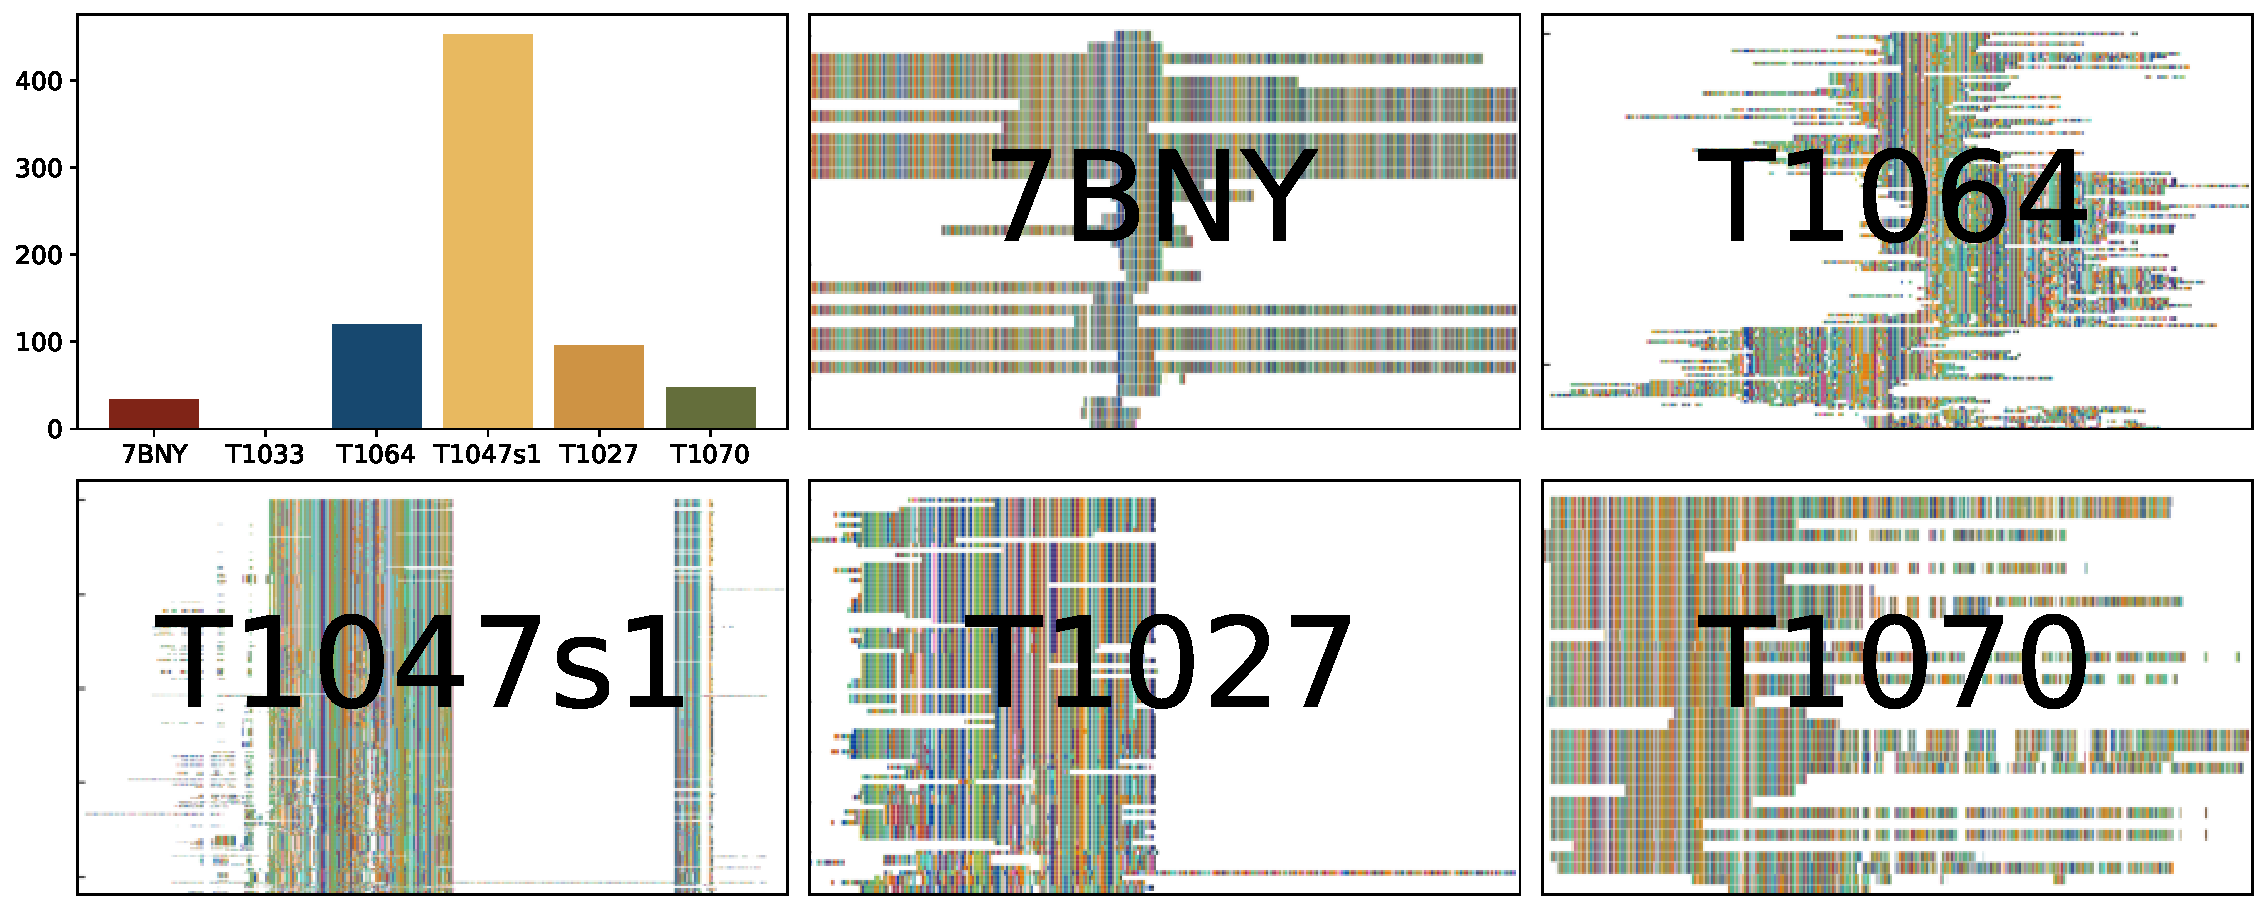
\includegraphics[width=\textwidth]{images/rna_virus_hits_with_images.pdf}
    \caption{\textbf{Visualization of homologs for rare RNA virus protein.}
    The upper left panel shows the distribution of homologs found in the collected data. Apart from T1033, which is a only 100 amino acid long short peptide,all other RdRPs have at least 40 homologs in the databases. The MSAs of each RdRP are generated in the other 5 panels.}
    \label{fig:rna-virus-hits}
  \end{figure}
  \restoregeometry
\end{figpage}
\clearpage
\pagebreak
